% =============================================================================
% PX4 + ROS 2 con px4_examples — Vespo UAV
%
% Compilar:  latexmk -pdf main.tex      (o pdflatex dos veces, por los índices)
% Necesita:  texlive-latex-extra texlive-lang-spanish texlive-pictures
%            texlive-fonts-recommended
%
% Cada sección vive en secciones/NN_nombre.tex. Todo lo que se cita del código
% sale de src/px4_examples/src/*.cpp.
% =============================================================================
% (el \documentclass va en cada presentación)

\usepackage[utf8]{inputenc}
\usepackage[T1]{fontenc}
\usepackage[spanish,es-nodecimaldot,es-noshorthands]{babel}
\usepackage{amsmath,amssymb}
\usepackage{booktabs}
\usepackage{graphicx}
\usepackage{xcolor}
\usepackage{listings}
\usepackage[most]{tcolorbox}
\usepackage{tikz}
\usetikzlibrary{arrows.meta,positioning,shapes.geometric,shapes.misc,calc,fit,backgrounds,decorations.pathreplacing}
\usepackage{multicol}
\usepackage{pifont}
% Lo que imprime vespo en la terminal
\DeclareUnicodeCharacter{2714}{\ding{51}}
\DeclareUnicodeCharacter{2718}{\ding{55}}
\DeclareUnicodeCharacter{2500}{\textendash}

\graphicspath{{img/}{img/px4docs/}{img/render/}{../../../x500_retos/docs/img/}}

% --- Tema: el de la intro a ROS2 ---------------------------------------------
\usetheme{default}
\useoutertheme{infolines}
\setbeamertemplate{headline}{}
\setbeamercolor{author in head/foot}{fg=black,bg=white}
\setbeamercolor{title in head/foot}{fg=blue!70!black,bg=white}
\setbeamercolor{date in head/foot}{fg=black,bg=white}
\setbeamercolor{section in toc}{fg=blue!70!black}
\setbeamertemplate{section in toc}[circle]
\setbeamercolor{frametitle}{fg=black,bg=white}
\setbeamerfont{frametitle}{size=\Large}
\setbeamertemplate{frametitle}{%
  \vskip0.4em
  \begin{beamercolorbox}[wd=\paperwidth,leftskip=0.3em,rightskip=0.3em]{frametitle}%
    \usebeamerfont{frametitle}\insertframetitle\hfill
    \raisebox{-0.45em}{
\includegraphics[height=1.6em]{vespo_logo}}%
  \end{beamercolorbox}}
\setbeamertemplate{caption}[numbered]
\setbeamertemplate{itemize items}[circle]
\setbeamercolor{itemize item}{fg=blue!70!black}
\setbeamercolor{enumerate item}{fg=blue!70!black}

% --- Colores y cajas -------------------------------------------------------------
\definecolor{azul}{RGB}{40,80,180}
\definecolor{azulclaro}{RGB}{232,238,252}
\definecolor{verde}{RGB}{0,128,0}
\definecolor{verdeclaro}{RGB}{236,250,236}
\definecolor{rojo}{RGB}{190,30,30}
\definecolor{naranja}{RGB}{230,120,10}
\definecolor{gris}{RGB}{110,110,110}

% Idea clave: caja azul redondeada con sombra.
\newtcolorbox{idea}[1][]{enhanced,colback=azulclaro,colframe=azul!40,arc=2mm,
  boxrule=0.4pt,drop shadow,left=1.5mm,right=1.5mm,top=1mm,bottom=1mm,#1}
% Ojo: lo que suele salir mal.
\newtcolorbox{ojo}[1][]{enhanced,colback=red!5,colframe=rojo!60,arc=2mm,boxrule=0.4pt,
  drop shadow,left=1.5mm,right=1.5mm,top=1mm,bottom=1mm,
  title={\small\bfseries Ojo},fonttitle=\small,coltitle=white,colbacktitle=rojo!80,#1}
% Salida de terminal: barra verde con el comando.
\newtcolorbox{terminal}[1]{enhanced,colback=verdeclaro,colframe=verde,arc=1mm,boxrule=0.6pt,
  title={\ttfamily\small #1},fonttitle=\ttfamily\small,coltitle=white,colbacktitle=verde,
  left=1mm,right=1mm,top=0.5mm,bottom=0.5mm,fontupper=\ttfamily\scriptsize}

% --- Código ----------------------------------------------------------------------
\renewcommand{\lstlistingname}{Código}
\lstset{
  basicstyle=\ttfamily\scriptsize,
  keywordstyle=\color{azul}\bfseries,
  commentstyle=\color{gris}\itshape,
  stringstyle=\color{verde},
  frame=single, rulecolor=\color{black},
  breaklines=true, columns=fullflexible, keepspaces=true,
  showstringspaces=false, captionpos=b, tabsize=2,
  xleftmargin=2pt, xrightmargin=2pt, aboveskip=4pt, belowskip=2pt,
  literate=
    {á}{{\'a}}1 {é}{{\'e}}1 {í}{{\'i}}1 {ó}{{\'o}}1 {ú}{{\'u}}1
    {Á}{{\'A}}1 {É}{{\'E}}1 {Í}{{\'I}}1 {Ó}{{\'O}}1 {Ú}{{\'U}}1
    {ñ}{{\~n}}1 {Ñ}{{\~N}}1 {ü}{{\"u}}1 {¿}{{?`}}1 {¡}{{!`}}1
    {°}{{$^\circ$}}1 {²}{{$^2$}}1 {·}{{$\cdot$}}1
    {→}{{$\rightarrow$}}2 {←}{{$\leftarrow$}}2 {≈}{{$\approx$}}1
    {▲}{{$\blacktriangle$}}1 {►}{{$\blacktriangleright$}}1 {│}{{|}}1 {─}{{-}}1
    {┌}{{+}}1 {┐}{{+}}1 {└}{{+}}1 {┘}{{+}}1 {├}{{+}}1 {┤}{{+}}1 {┼}{{+}}1
}
\lstdefinestyle{cpp}{language=C++,morekeywords={override,nullptr,constexpr,auto}}
\lstdefinestyle{bash}{language=bash,morekeywords={ros2,vespo,colcon}}
\lstdefinelanguage{yaml}{morecomment=[l]\#,morestring=[b]"}

% --- Atajos ---------------------------------------------------------------------
\newcommand{\cmd}[1]{\texttt{#1}}
\newcommand{\ok}{{\color{verde}\checkmark}}
\newcommand{\mal}{{\color{rojo}$\times$}}

% Al empezar cada sección: el contenido con la sección actual resaltada.
\AtBeginSection[]{%
  \begin{frame}{Contenido}
    \begin{multicols}{2}\scriptsize
      \tableofcontents[currentsection]
    \end{multicols}
  \end{frame}}

% Láminas que se arman paso a paso: en TikZ, "visible on=<3->" muestra un
% nodo desde el paso 3 y "alt=<2>{fill=...}{fill=...}" lo resalta en el paso 2.
\tikzset{
  invisible/.style={opacity=0,text opacity=0},
  visible on/.style={alt={#1{}{invisible}}},
  alt/.code args={<#1>#2#3}{\alt<#1>{\pgfkeysalso{#2}}{\pgfkeysalso{#3}}},
}
\newcommand{\credito}[1]{{\tiny\color{gris}#1}}

% El x500 recortado (tools/renders_x500.py + tools/recortar_iconos.py).
% \dronarriba{ancho}: visto desde arriba, la nariz hacia arriba de la imagen.
% Para girarlo a un yaw (0 = norte, positivo hacia el este) en TikZ: \node[rotate=-yaw].
\newcommand{\dronarriba}[1]{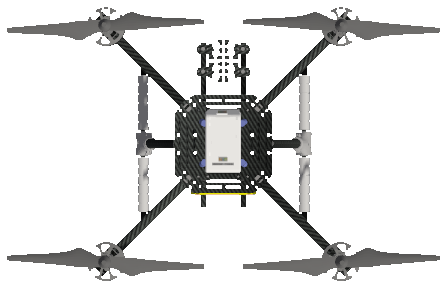
\includegraphics[width=#1]{x500_icono}}
\newcommand{\dronlado}[1]{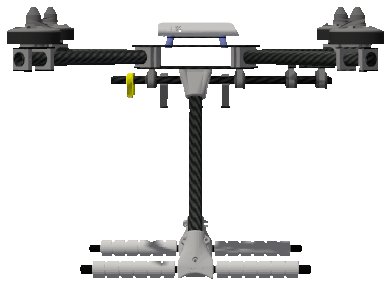
\includegraphics[width=#1]{x500_lado_icono}}
